\documentclass{homework}

\title{Homework 4}
\author{Kevin Evans}
\studentid{11571810}
\date{September 21, 2020}
\setclass{Physics}{341}
\usepackage{amssymb}
\usepackage{mathtools}

\usepackage{amsthm}
\usepackage{amsmath}
\usepackage{slashed}
\usepackage{relsize}
\usepackage{threeparttable}
\usepackage{float}
\usepackage{booktabs}
\usepackage{boldline}
\usepackage{changepage}
\usepackage{physics}
\usepackage[inter-unit-product =\cdot]{siunitx}
\usepackage{setspace}

\usepackage[makeroom]{cancel}
%\usepackage{pgfplots}

\usepackage{enumitem}
\usepackage{times}

\usepackage{calligra}
\DeclareMathAlphabet{\mathcalligra}{T1}{calligra}{m}{n}
\DeclareFontShape{T1}{calligra}{m}{n}{<->s*[2.2]callig15}{}
\newcommand{\scriptr}{\mathcalligra{r}\,}
\newcommand{\boldscriptr}{\pmb{\mathcalligra{r}}\,}

\begin{document}
	\maketitle
	\begin{enumerate}
		\item For a sphere with charge density $\rho = k r^2$, the charge enclosed within a Gaussian surface is \begin{align*}
			q_\mathrm{enc} & = \int_{0}^{r} \rho(r') \dd{\tau} \\
				& = 4 k \pi \int_0^r r'^4 \dd{r'} \\
				& = \frac{4 k \pi r^5 }{5}
		\end{align*}
		From Gauss' law, since the electric field is outward and uniform in the $\uvec{r}$ direction as the charge density only depends on $r$, \begin{align*}
			\bvec{E} \cdot \int_S \dd{\bvec{a}} & = \frac{ q_\mathrm{enc} }{\epsilon_0} \\
			\bvec{E} & = \frac{4 k \pi r^5}{5 \epsilon_0} \left(\frac{4}{3} \pi r^3\right)^{-1} \uvec{r} \\
				& = \frac{3 r^2}{5 \epsilon_0} \uvec{r}
		\end{align*}
	
		\item \begin{enumerate}
			\item[i.] Within the inner cylinder, the enclosed charge of a Gaussian surface is \begin{align*}
				q_\mathrm{enc} & = \int \rho(s') \dd{\tau} \\
					& = 2 \pi k L \int_0^s s'^2 \dd{s'} \\
					& = \frac{2 \pi k L s^3}{3}
				\intertext{As the electric field will point cylindrically outward in $\uvec{s}$ and from Gauss' law,}
				\bvec{E} & = \frac{2 \pi k L s^3}{3 \epsilon_0} \frac{1}{2 \pi s L} \uvec{s} \\
					& = \frac{k s^2}{3 \epsilon_0} \uvec{s}
			\end{align*}
			
			\item[ii.] Between the cylinders, the enclosed charge will be the entirety of the inner cylinder, \begin{align*}
				q_\mathrm{enc} & = \frac{2 \pi k L a^3}{3}
				\intertext{From a similar approach as above, }
				\bvec{E} & = \frac{ka^3}{3 \epsilon_0 s}
			\end{align*}
			
			\item[iii.] Outside the cylinders, the enclosed charge is zero and there will be no electric field, $\bvec{E} = 0$.
			
			% TODO: \usepackage{graphicx} required
			\begin{center}
				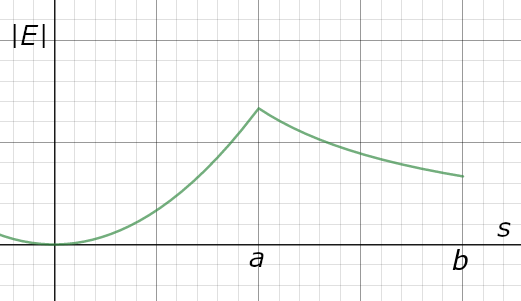
\includegraphics[width=0.7\linewidth]{hw4plot}
			\end{center}
			
		\end{enumerate}
	
		\item Integrating the electric field along $s$, \begin{align*}
			V & = - \frac{k}{3 \epsilon_0} \left[ \int_{0}^{a} s^2 \dd{s} + a^3 \int_a^b s^{-1} \dd{s}   \right] \\
				& = - \frac{k}{3 \epsilon_0} \left[ \frac{a^3}{3} + a^3 \ln( \frac{b}{a} ) \right] \\
				& = -\frac{ka^3}{3 \epsilon_0} \left[
					\frac{1}{3} + \ln(\frac{b}{a})
				\right]
		\end{align*}
	
	
		\item The distance between a segment of the charged ring and the observation point is given as \begin{align*}
			\abs{\boldscriptr} & = \left(z^2 + R^2\right)^{1/2}
			\intertext{Using the distance above, the potential is}
			V(z) & = \frac{\lambda}{4 \pi \epsilon_0} \int_0^{2 \pi} \left(z^2 + R^2\right)^{-1/2} R \dd{\phi} \\
				& = \frac{\lambda R}{2 \epsilon_0 \left(z^2 + R^2\right)}
			\intertext{From this potential, the electric field can be determined using the gradient of $V$,}
			\bvec{E} & = - \grad{V} = - \pdv{z} V(z) \\
				& = -\frac{ \lambda R }{2 \epsilon_0} \left( - \frac{1}{2\left(z^2 + R^2\right)^{3/2}} \right) \left(2z\right) \uvec{z} \\
				& = \frac{\lambda Rz}{2 \epsilon_0 \left(z^2 + R^2\right)^{3/2}} \uvec{z}
		\end{align*}
	
		\pagebreak
		
		\item From the potential \[ V(\bvec{r}) = A \frac{ e^{-\lambda r}}{r}\]
		The electric field $\bvec{E}(\bvec{r})$ is found using the negative gradient \begin{align*}
			\bvec{E} & = - \grad[ A \frac{ e^{-\lambda r}}{r} ] \\
				& = - A \pdv{r} \frac{e^{-\lambda r}}{r} \uvec{r} = A \left[ \frac{\lambda e^{-\lambda r}}{r} + \frac{e^{-\lambda r}}{r^2}\right] \uvec{r} \\
				& = \frac{ Ae^{-\lambda r}}{r} \left(\lambda + \frac{1}{r}\right) \uvec{r} \\
			\intertext{The charge density is given by Gauss's law, }
			\rho(r) & = \epsilon_0 \div{\bvec{E}} = \frac{ \epsilon_0 }{r^2} \pdv{r} \left(r^2 E_r\right) \\
				& = \frac{A\epsilon_0}{r^2} \div[
					e^{-\lambda r}\left(\lambda r + 1\right) \left(\frac{ \uvec{r} }{r^2}\right)
				]
			\intertext{Applying the product rule and delta properties,}
				& = \frac{A\epsilon_0}{r^2} \left[
					4 \pi e^{-\lambda r} \left(\lambda r + 1\right) \delta(r) + \frac{\bvec{r}}{r^2}  \cdot
					\grad[e^{-\lambda r} \left(\lambda r + 1\right)]
				\right] \\
				& = \frac{A\epsilon_0}{r^2} \left[
				4 \pi e^{-\lambda r} \left(\lambda r + 1\right) \delta({r}) +
				\frac{1}{r^2} 
				\left(
					\lambda e^{-\lambda r}
					- \lambda e^{-\lambda r} \left(\lambda r + 1\right)
				\right)
				\right] \\
				& = \frac{ A\epsilon_0 }{r^2} \left(e^{-\lambda r}\right) \left[4 \pi (\lambda r + 1)\delta(r)
				- \frac{ \lambda^2 }{r}
				 \right]
		\end{align*}
	\end{enumerate}
\end{document}